\documentclass[10pt, oneside]{article}
\usepackage[a4paper, total={5.5in, 9in}]{geometry}
\usepackage[ngerman]{babel}
\usepackage{import}

\import{../../.texit/include}{preamble}

\title{Einführung in die Künstliche Intelligenz\\[15pt]\Large{Übungsblatt 2}\\[10pt]\Large{SoSe 2025}}
\author{Volodymyr But\\[10pt]Hochschule Trier}
\date{}

% - - - - - - - - - - - - - - - - - - - - - - - - - - - - - - - - - - - - - - %

\begin{document}

\maketitle
\vspace{25px}

\section{1\ \ \ Definitionen}

\begin{enumerate}[(a)]
    \item \textbf{Hypothese} ist eine Funktion, die aus Eingabe und
        Trainingsdaten, die die Beziehung zwischen Eingabe und Ausgabe
        definieren, eine approximierte Ausgabe erzeugt.

    \item \textbf{Hypothesenraum} ist eine Menge an Funktionen, aus denen eine
        Hypothese ausgew"ahlt wird.

    \item \textbf{Klassifikation} ist eine Zuordnung einer Art von Ausgangswert
        zu einem gegebenen Eingangswert.

    \item \textbf{Regression} ist eine Menge statistischer Verfahren zur
        Bestimmung der Beziehungen zwischen einer Ausgabe und einer oder
        mehreren Features (Eingabe).

    \item \textbf{Ockhams Razor} ist das Problemlösungsprinzip, das die Suche
        nach Erklärungen empfiehlt, die aus der kleinstmöglichen Menge von
        Elementen bestehen.
\end{enumerate}

\section{2\ \ \ Lernformen}

\begin{itemize}
    \item Wettervorhersage
        \begin{itemize}
            \item unüberwachtes Lernen
            \item Daten sind unbeschriftet
            \item Machine erkennt die Muster in der Eingabe selbst"andig.
        \end{itemize}

    \item Empfehlungssysteme (z.B. Youtube, Spotify oder Netflix)
        \begin{itemize}
            \item verstärkendes Lernen
            \item Maschine sagt die Bewertung eines Nutzers für ein Foto, ein
                Video oder einen Film voraus.
            \item System erh"alt Pluspunkte, wenn ein Nutzer eine Empfehlung
                anschaut oder wenn dem Nutzer die Empfehlung gefallen hat, und
                Minuspunkte, wenn er die Empfehlung komplett ignoriert.
            \item System lernt durch Belohnung und Bestrafung, bessere
                Entscheidungen zu treffen.
        \end{itemize}

    \item Spam-Filter
        \begin{itemize}
            \item überwachtes Lernen.
            \item System lernt aus markierten E-Mails, Spam-Briefe zu erkennen
        \end{itemize}
\end{itemize}

\section{3\ \ \ Aufteilung von Daten}

\begin{enumerate}[(a)]
    \item nicht sinnvoll. Die Trainingsdaten enthalten ausschlie{\ss}lich
        Spam-Emails. Es wird somit nicht "uberpr"uft, ob das System
        f"alschlicherweise auch normale E-Mails als Spam klassifiziert.
    \item Der Fall ist besser, da die Testdaten nun sowohl Spam-E-Mails als
        auch normale Nachrichten enthalten. Jedoch sind die Menge der Testdaten 
        und die Menge der Trainingsdaten sind nicht disjunkt, also kann es zu
        einer Überschätzung der Modellleistung kommen. Dies liegt daran, dass
        das Modell während des Trainings möglicherweise bereits ähnliche oder
        identische Daten gesehen hat, was die Generalisierungsfähigkeit auf
        völlig neue, unbekannte Beispiele einschränken könnte. Um eine
        realistischere Einschätzung der Modellgüte zu erhalten, wäre es daher
        sinnvoll, strikt disjunkte Trainings- und Testmengen zu verwenden.
\end{enumerate}

\section{4\ \ \ Entscheidungsb"aume anwenden}

\begin{enumerate}[(a)]
    \item No \\[5pt]
          Yes \\[5pt]
          Yes
    \item Patrons? Some oder None
    \item Patrons?: Full \\[5pt]
          Wait Estimate?: 30-60 \\[5pt]
          Alternate?: No \\[5pt]
          Reservation?: No \\[5pt]
          Bar?: Yes
\end{enumerate}

\section{5\ \ \ Entscheidungsb"aume erstellen}

Siehe Abbildungen 5.1, 5.2 und 5.3

\begin{figure}[p]
    \centering
    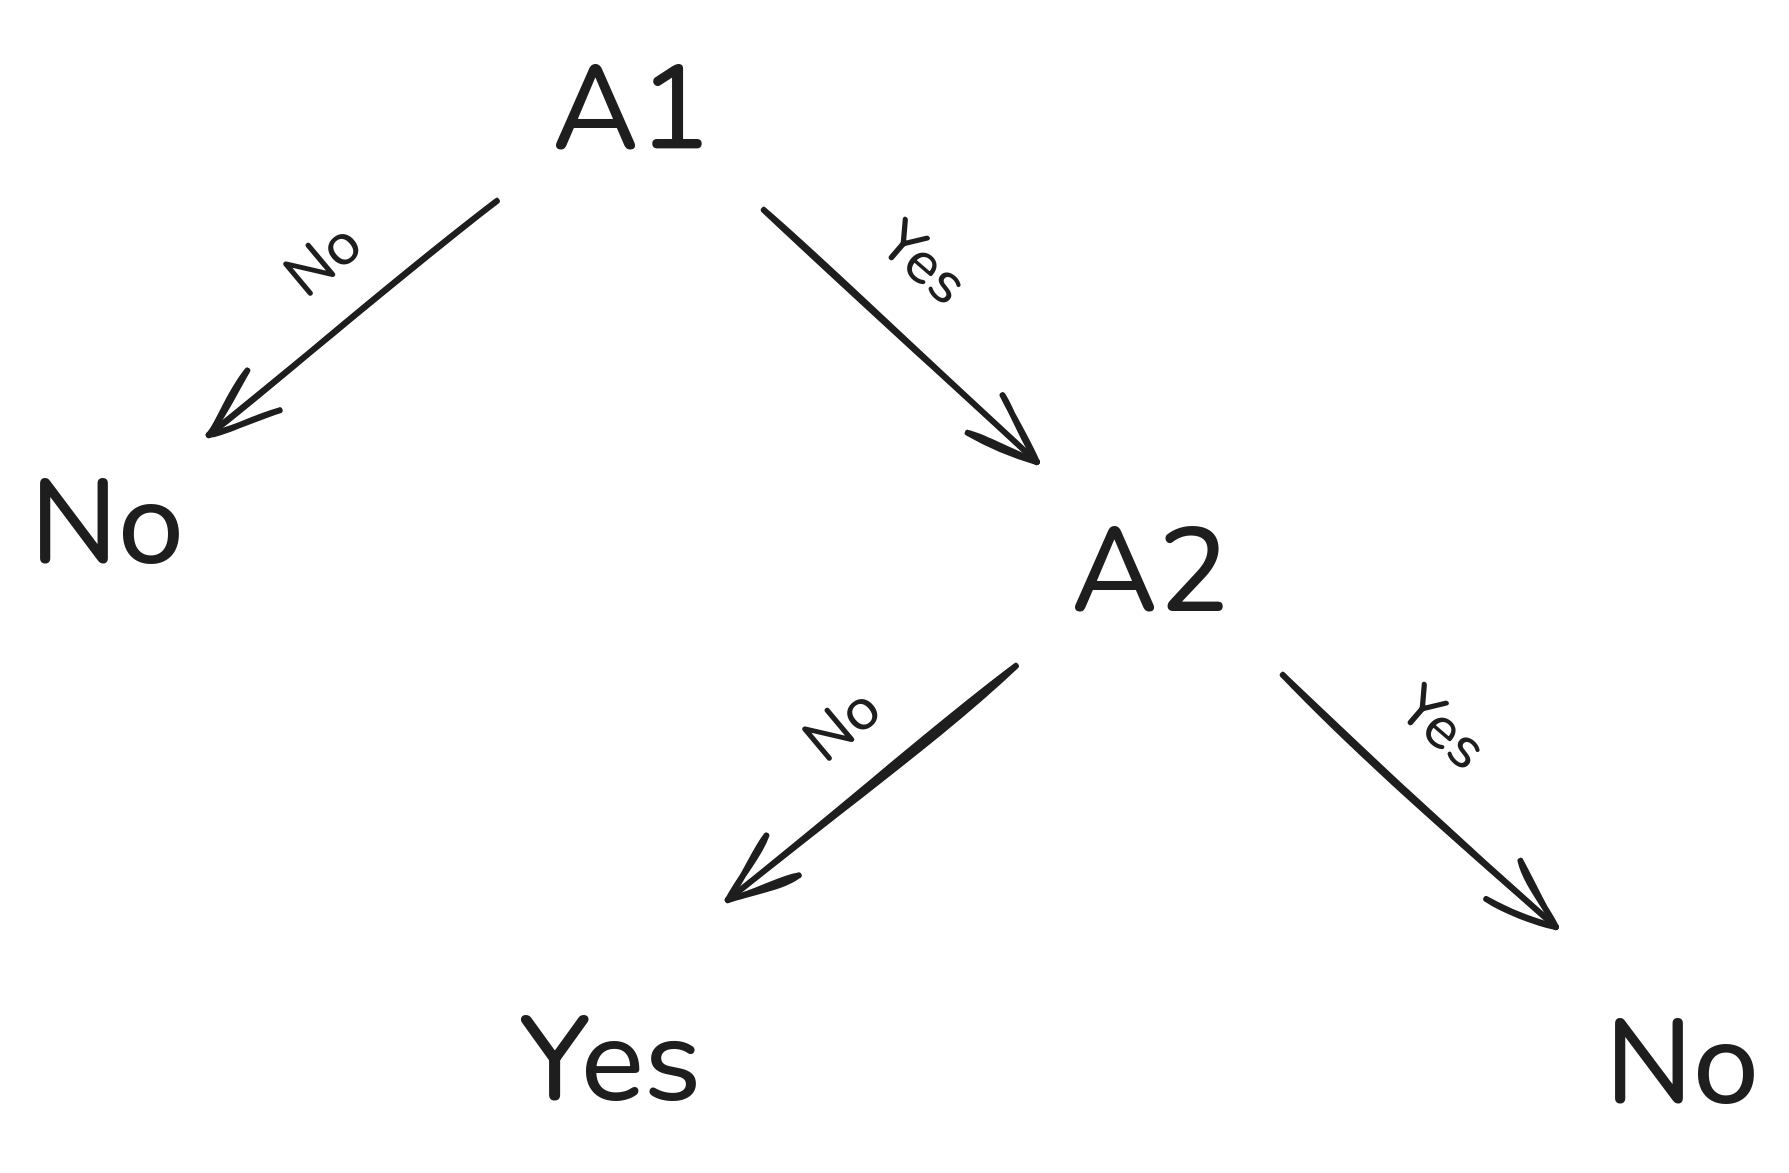
\includegraphics[width=1\textwidth]{./assets/ueb02-5-1.png}
    \caption{(a)}
\end{figure}

\FloatBarrier

\begin{figure}[p]
    \centering
    \centering
    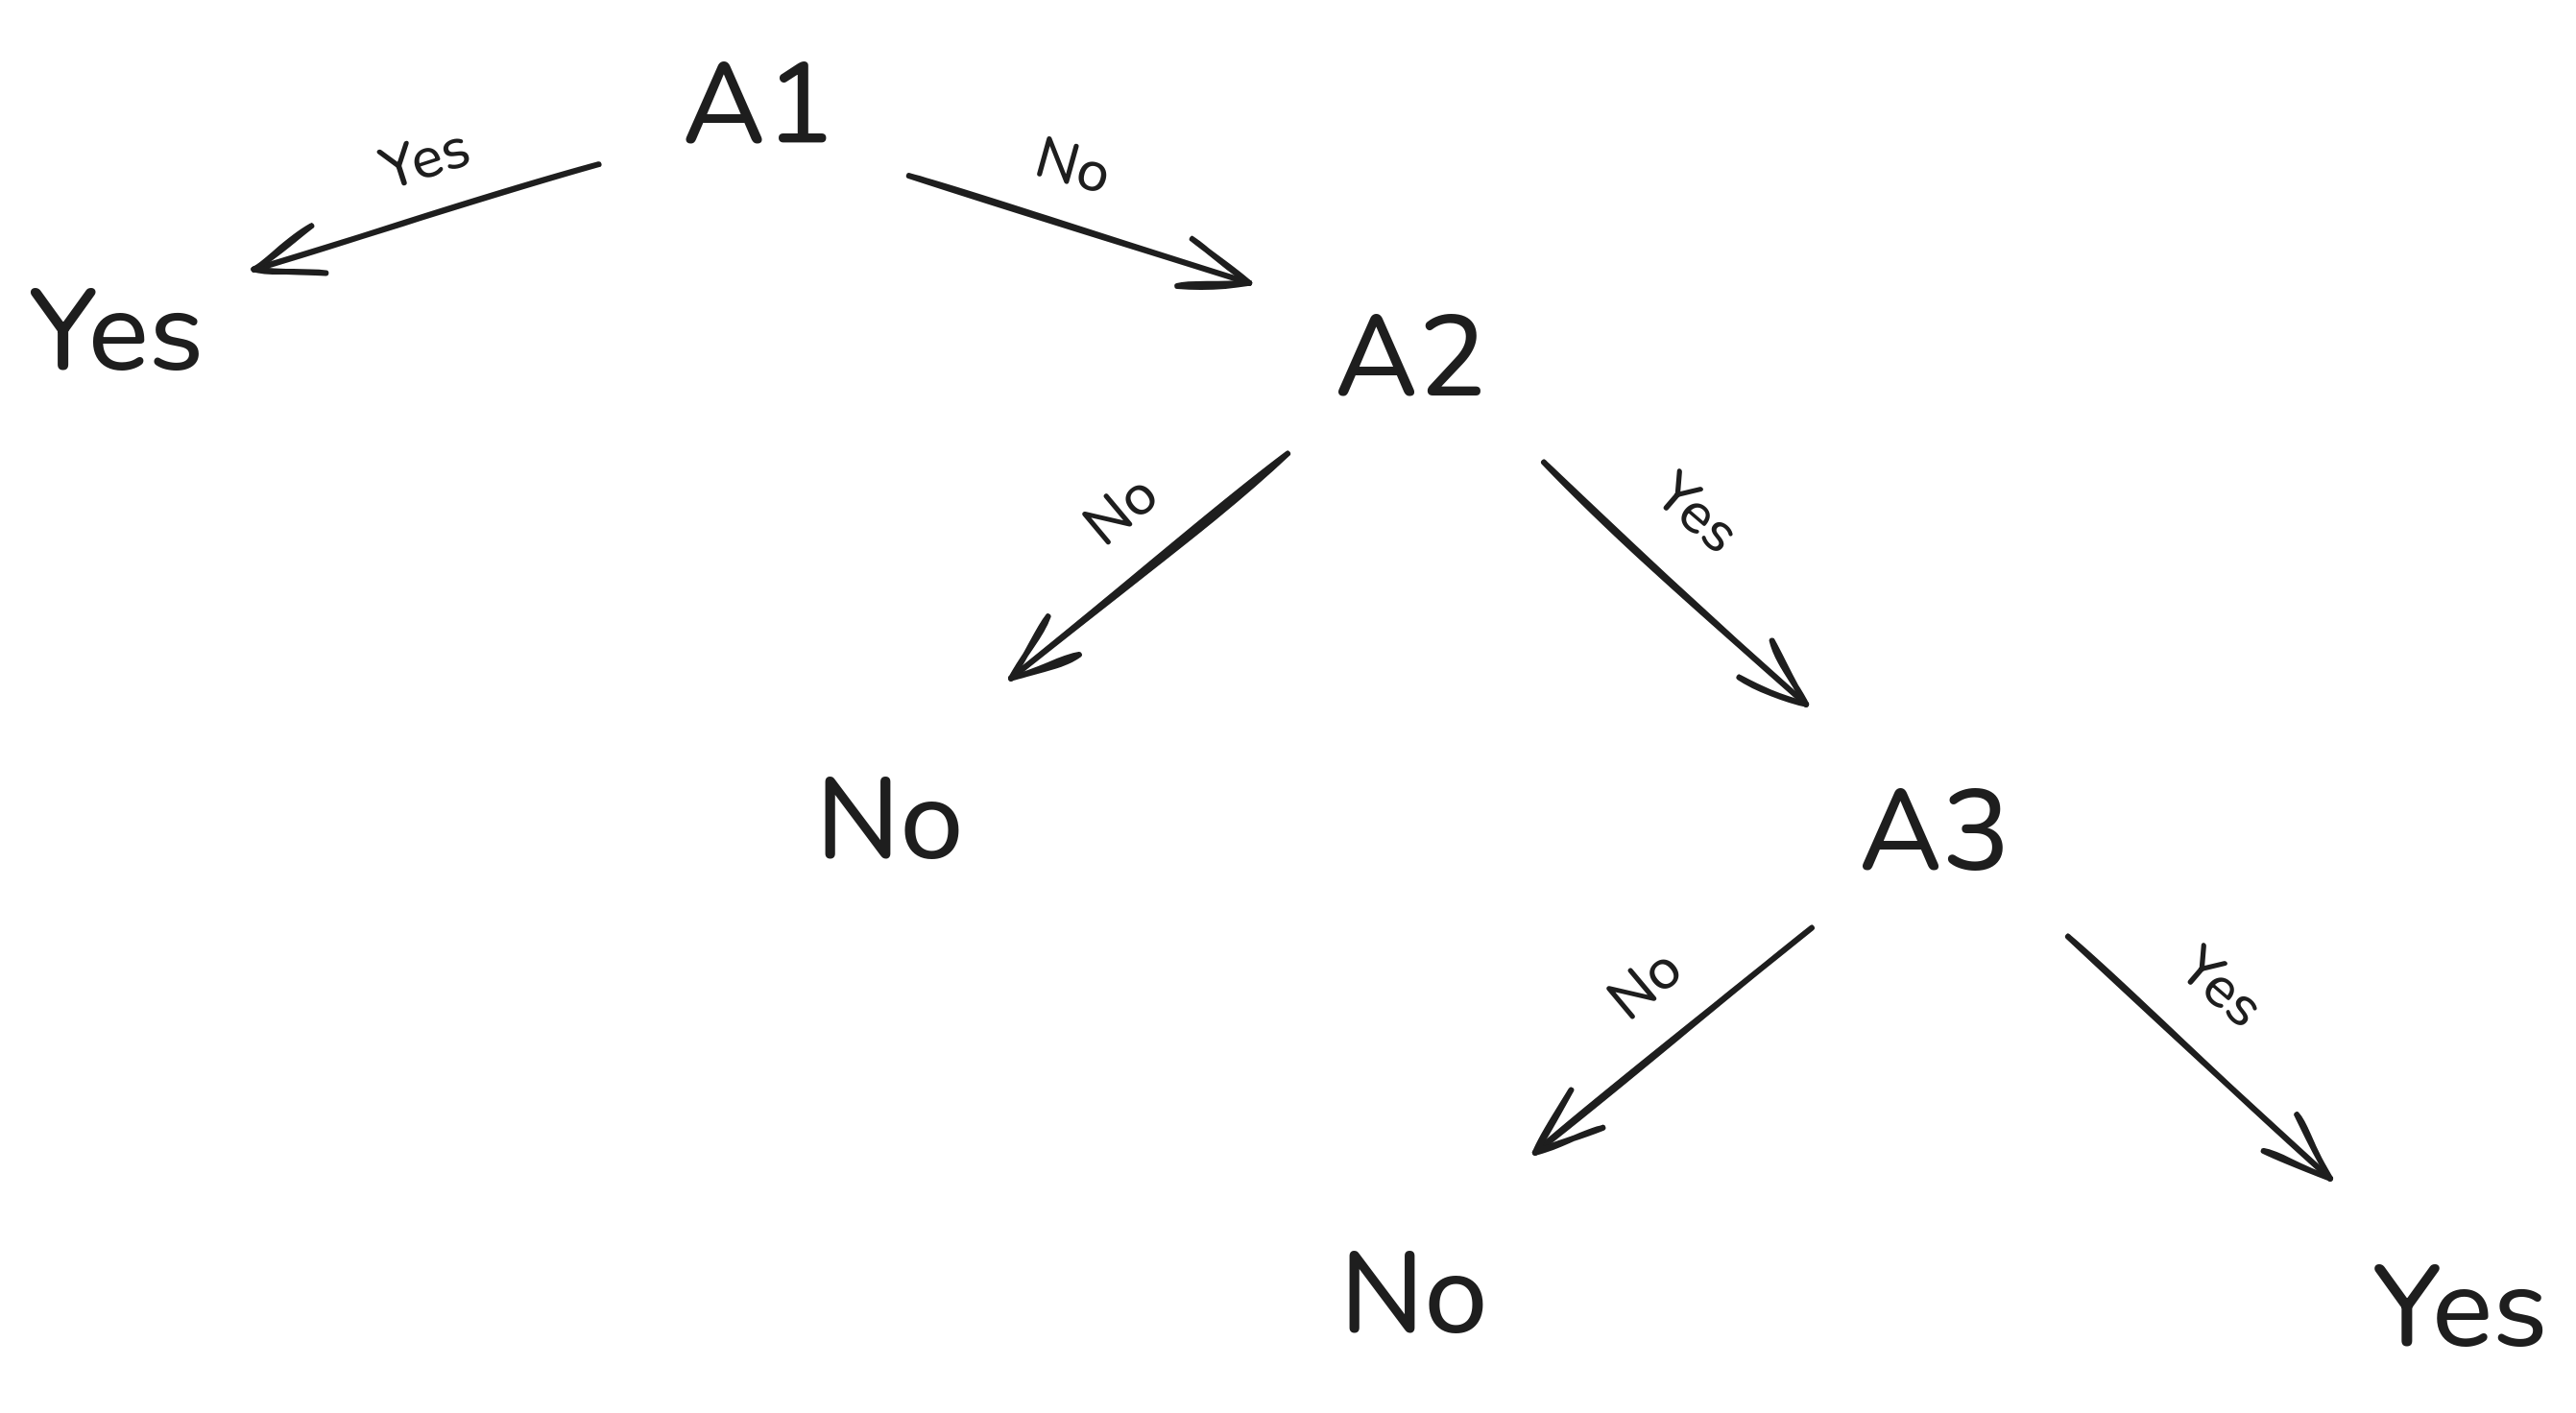
\includegraphics[width=1\textwidth]{./assets/ueb02-5-2.png}
    \caption{(b)}
\end{figure}

\FloatBarrier

\begin{figure}[p]
    \centering
    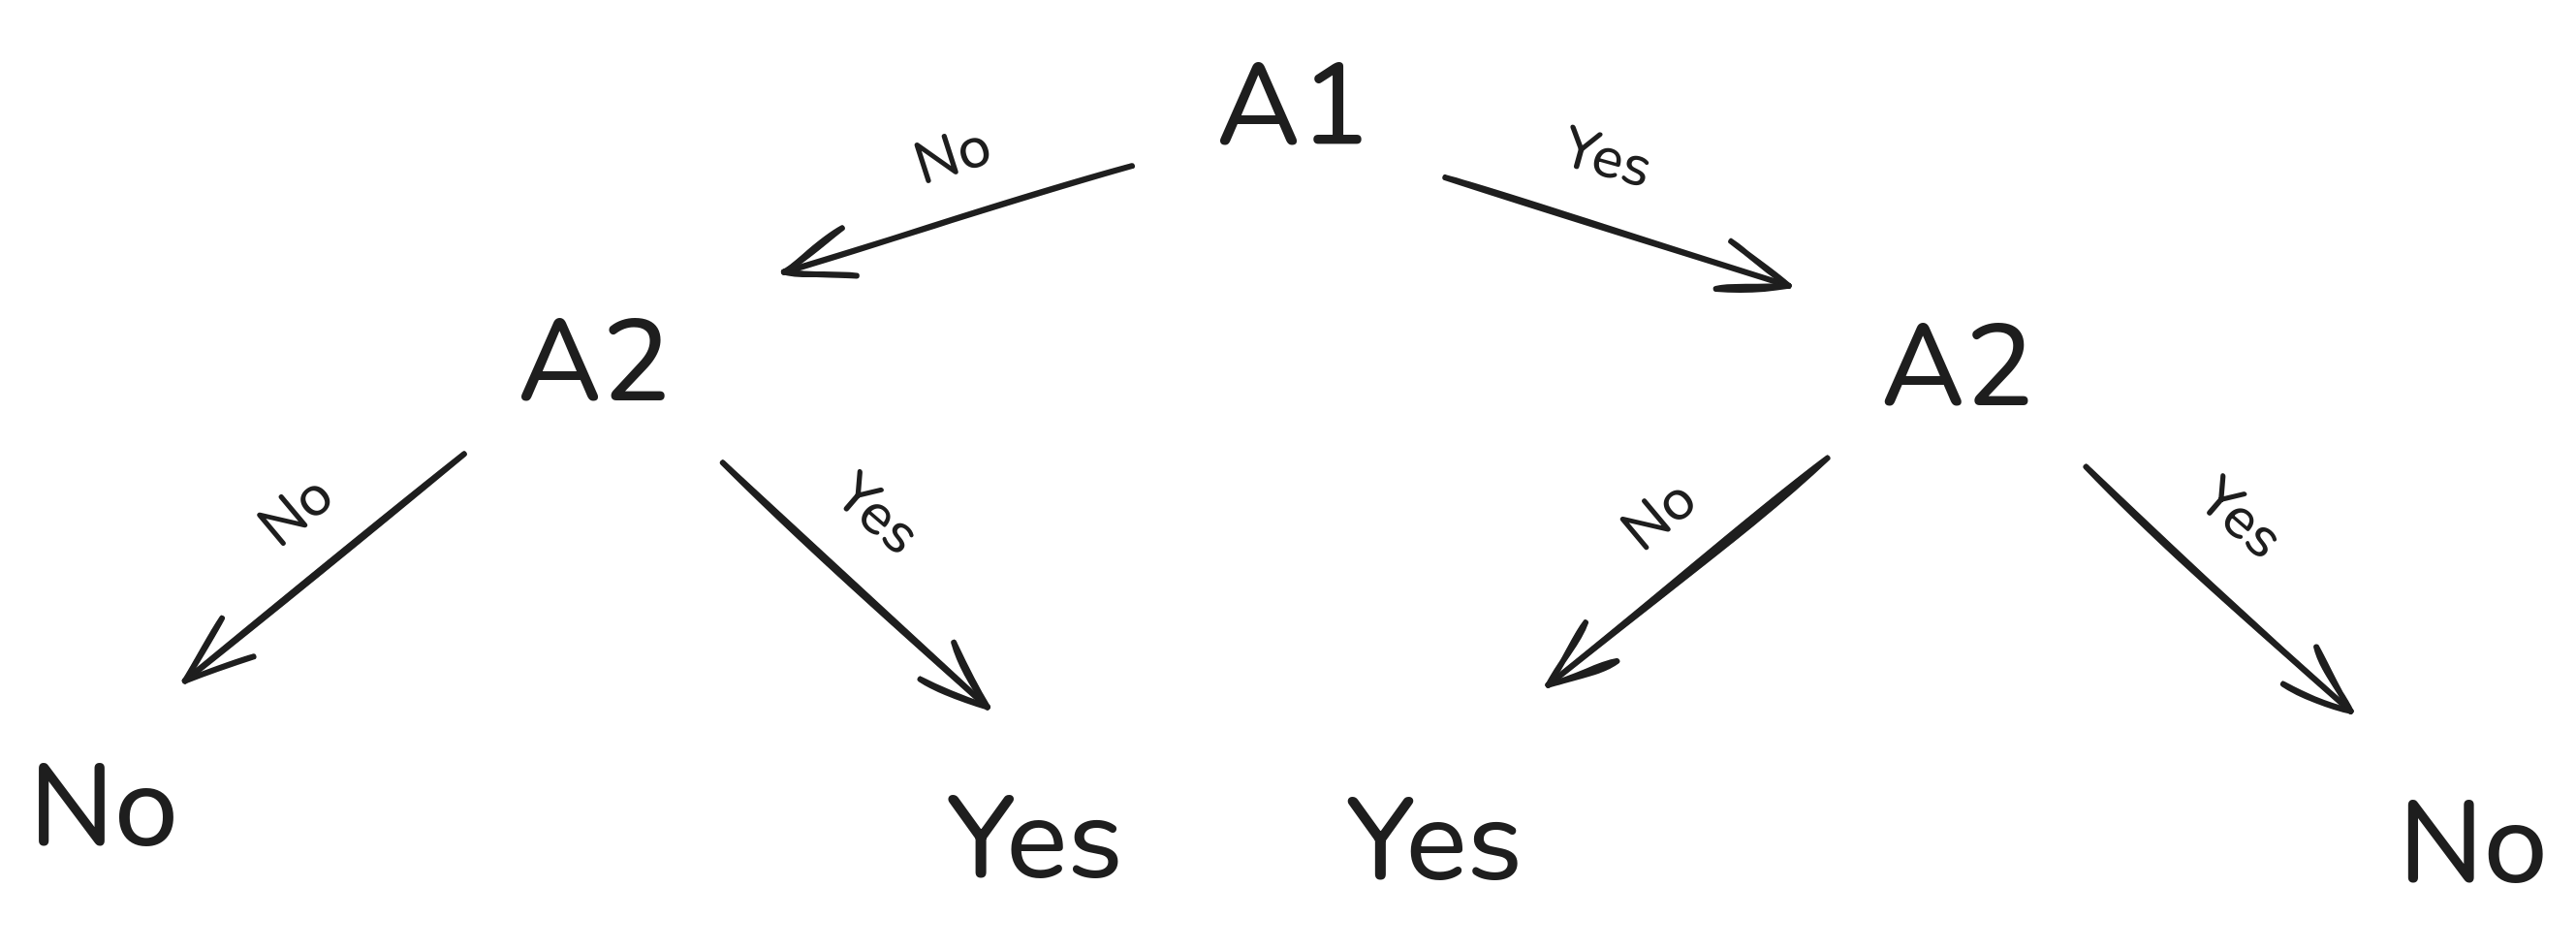
\includegraphics[width=1\textwidth]{./assets/ueb02-5-3.png}
    \caption{(c)}
\end{figure}

\FloatBarrier

\end{document}
